\documentclass[t,usepdftitle=false]{beamer}

\usepackage[utf8]{inputenc}
\usetheme{Singapore}
\usepackage{xcolor}
\setbeamertemplate{footline}[frame number]

\title[IFT3515]{IFT 3515\\Fonctions à plusieurs variables\\Optimisation sous contraintes\\Méthodes de projection}
\author[Fabian Bastin]{Fabian Bastin\\DIRO\\Université de Montréal}
\date{}

\usepackage{enumerate}
\usepackage[french]{babel}

\usepackage{easybmat}
\usepackage{graphicx}

\usepackage{amsmath}

\newtheorem{defn}{Définition}
\newtheorem{lem}{Lemme}
\newtheorem{thm}{Théorème}
\newtheorem{coro}{Corollaire}

\def\red{\color{red}}
\def\blue{\color{blue}}

\def\co{\mathcal{o}}

\def\RR{\mathbb{R}}

\def\cB{\mathcal{B}}
\def\cC{\mathcal{C}}
\def\cL{\mathcal{L}}
\def\cN{\mathcal{N}}
\def\cR{\mathcal{R}}
\def\cS{\mathcal{S}}
\def\cT{\mathcal{T}}
\def\cX{\mathcal{X}}

\def\bu{\boldsymbol{u}}

\setbeamertemplate{footline}[frame number]

\begin{document}
\frame{\titlepage}

\begin{frame}
\frametitle{Cadre de travail}

Jusqu'à présent, nous n'avons considéré que des problèmes d'optimisation sans contraintes.
La plupart des problèmes pratiques présentent toutefois des contraintes, et il convient d'adapter nos méthodes pour en tenir compte.

\mbox{}

Nous considérons dans un premier temps des contraintes simples, définissant une région convexe.

\mbox{}

Soit le programme
$$
\min_{x \in \cX} f(x)
$$
où $\cX \subseteq \mathbb{R}^n$ est l'ensemble réalisable, supposé fermé et non vide.

\end{frame}

\begin{frame}
\frametitle{Ensemble convexe}

De plus, nous supposons pour le moment que $\cX$ est convexe, et qu'il est relativement aisé de projeter n'importe quel point sur cet ensemble.

\mbox{}

Rappel: un ensemble $\cX$ est convexe ssi toute combinaison convexe de points dans $\cX$ est également dans $\cX$:
$$
\forall\, x, y \in \cX,\ \forall\, \lambda \in [0,1],\ \lambda x + (1-\lambda)y \in \cX.
$$
\end{frame}
	
\begin{frame}
\frametitle{Conditions d'optimalité au premier ordre}

Lecture suggérée: Nocedal et Wright, Chapitre 12.

\mbox{}

Nous devons tout d'abord revoir nos conditions d'optimalité pour le cas contraint.

\mbox{}

\begin{thm}[Condition nécessaire au premier ordre]
Soit $f$ continûment différentiable sur $\cX \in \mathbb{R}^n$, avec $\cX$ fermé et non vide.
Si $x^*$ est un minimum local de $f$, alors
\[
-\nabla_x f(x^*) \in \mathcal{N}_{\mathcal{X}}(x^*),
\]
où $\mathcal{N}_{\cX(x^*)}$ est le cône normal à $\mathcal{X}$ en $x^*$.
\end{thm}	

\mbox{}

Si $f$ est convexe, la condition est nécessaire et suffisante.

\end{frame}

\begin{frame}
\frametitle{Définitions}

\begin{defn}[Cône]
Un sous-ensemble $\cC$ d'un espace vectoriel $V$ est un {\red cône} linéaire
ssi	$\alpha x$ appartient à $\cC$ pour tout $x \in C$ et tout scalaire $\alpha > 0$.\\
Le cône est pointé si $\forall \alpha \geq 0,\ \alpha x \in \cC$.
\end{defn}

\mbox{}
	
\begin{defn}[Cône convexe]
Un {\red cône convexe} $\cC$ est un cône fermé sous les combinaisons convexes, i.e. ssi $\alpha x + \beta y \in \cC$, $\forall \alpha,\ \beta > 0$, avec $\alpha + \beta = 1$.
\end{defn}

\end{frame}

\begin{frame}
\frametitle{Cône tangent et cône normal}

\begin{defn}[Vecteur tangent]
Un vecteur $w \in \mathbb{R}^n$ est tangent à $\cX$ en $x \in \cX$ si pour toute séquence de vecteurs $\lbrace x_i \rbrace$ avec $x_i \rightarrow x$ et $x_i \in \cX$, et toute séquence de scalaires positifs $t_i \downarrow 0$, il existe une séquence $w_i \rightarrow w$ telle que $x_i + t_iw_i \in \cX$ pour tout $i$.
\end{defn}	
	
\begin{defn}[Cône tangent]
Le {\red cône tangent $T_{\cX}(x)$} est la collection des vecteurs tangents à $\cX$ en $x$.
\end{defn}	

\begin{defn}[Cône normal]
Le {\red cône normal $N_{\cX}(x)$} est le complément orthogonal de $T_{\cX}(x)$, i.e.
\[
N_{\cX}(x) = \lbrace v\ |\ v^Tw \leq 0,\ \forall w \in T_{\cX}(x) \rbrace.
\]
\end{defn}	
	
\end{frame}

\begin{frame}
\frametitle{Cas convexe: cône normal}

La définition de cône normal peut être simplifiée si $\cX$ est convexe.
Nous avons en effet alors
$$
N_{\cX}(x) =
\begin{cases}
\left\lbrace v\ |\ v^T(x-x_0) \geq 0,\ \forall x_0 \in \cX \right\rbrace & \text{\ si\ } x \in \cX,\\
\emptyset & \text{\ sinon.}
\end{cases}
$$
	
\mbox{}

La condition nécessaire d'optimalité devient alors
$$	
\nabla f(x^*)^T (x-x^*) \geq 0\ \forall x \in \cX
$$.
	
%\mbox{}
	
Si $f$ est convexe (i.e. nous sommes dans le cadre de la programmation convexe), la condition est aussi suffisante.

\end{frame}

\begin{frame}
\frametitle{Cas convexe: cône tangent}

Dans le cas convexe, le cône tangent en $x \in \cX$ devient
$$
T_{\cX}(x) = cl\{ \theta(x_0-x) \,|\, \theta \geq 0 \mbox{ et } x_0 \in \cX \},
$$
où $cl\{\cS\}$ désigne la fermeture (closure) de l'ensemble $\cS$:
$$
cl\{\cS\} = \{ x \,|\, \forall\, \epsilon > 0,\, \cS \cap \cB(x,\epsilon) \ne \emptyset \}.
$$

\mbox{}

Décomposition de Moreau avec $y \in \cX$:
$$
x = P_{T_{\cX}(y)}(x) + P_{\cN_{\cX}(y)}(x).
$$

\end{frame}

\begin{frame}
\frametitle{Illustration graphique}
	
\begin{center}
	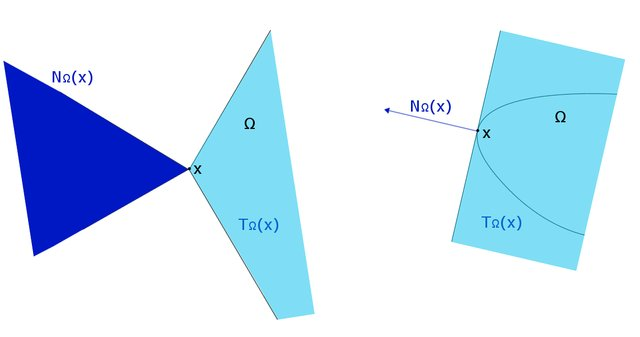
\includegraphics[width=0.9\textwidth]{Examples-of-the-tangent-and-normal-cones-of-given-convex-set-O_W640.jpg}
\end{center}
{\footnotesize{Source: Nikola Plivova et Petr Beremlijski, \textit{Proximal Bundle Method for Contact Shape Optimization Problem}, Advances in Electrical and Electronic Engineering 15(2), 2017.}}

\end{frame}

\begin{frame}
\frametitle{Cas tangent: interprétation}

Rappelons que $d$ est une direction réalisable en $x \in \cX$ s'il existe un scalaire $\alpha_{\max}$ tel que $x + \alpha d \in \cX$  pour tout $\alpha \in [0, \alpha_{\max}]$. 

\mbox{}

Le cône tangent peut encore être interpétré comme la fermeture du cône de toutes les directions réalisables.

\end{frame}

\begin{frame}
\frametitle{Théorème de projection}

Étant donné $x_0 \in \mathbb{R}^n$, nous voudrions identifier le point le plus proche de $x_0$ appartenant à $\cX$. Le théorème suivant caractérise ce point.

\begin{thm}[Projection pour des ensembles convexes]
Soit $x_0 \in \mathbb{R}^n$ et $\cX \subseteq \mathbb{R}^n$ un ensemble convexe, fermé et non vide.
$\overline{x} \in \cX$ résoud le problème
$$
\min_{x \in \cX} \frac{1}{2} \| x - x_0 \|_2^2
$$
si et seulement si, $\forall y \in \cX$.
$$
\langle \overline{x} - x_0, y - \overline{x} \rangle \geq 0
$$
De plus, la solution $\overline{x}$ existe toujours, et est unique.
\end{thm}
	
\end{frame}

\begin{frame}
\frametitle{Preuve}

Soit
$$
f(x) = \frac{1}{2} \| x - x_0 \|^2_2
$$
L'existence d'un minimum de $f(x)$ vient la compacité de l'ensemble
$$
\lbrace x \in \cX \,|\, \| x - x_0 \|_2 \leq \| \hat{x} - x_0 \|_2 \rbrace
$$
pour n'importe quel $\hat{x} \in \cX$.

\mbox{}

D'autre part, $f$ est strictement convexe, et donc admet un minimum unique, qui s'obtient en appliquant les conditions d'optimalité au premier ordre, ou
$$
\nabla f(x) = x - x_0.
$$

\end{frame}

\begin{frame}
\frametitle{Projection}

\begin{defn}[Projection]
Soit $\cX \subseteq \mathbb{R}^n$ un ensemble convexe, fermé et non vide.
La projection $P_{\cX}$ est le mapping $P_{\cX}: \mathbb{R}^n \rightarrow \cX$ donné par
$$
\| P_{\cX}-x \|_2^2 = \min_y \lbrace \| y - x \|_2^2 \,|\, y \in \cX \rbrace
$$
\end{defn}

\end{frame}

\begin{frame}
\frametitle{Contraintes de bornes}

Un des cas les plus simples est la situation où les variables de décision sont bornées inférieurement et supérieurement.
$$
\cX = \lbrace x \,|\, x_{\ell} \leq x \leq x_u \rbrace
$$
où les inégalités sont à comprendre composante par composante.

\mbox{}

Nous autorisons certaines composantes de $x_{\ell}$ à être égale à $-\infty$ et certaines composantes de $x_u$ à être égale à $+\infty$.

\mbox{}

Soit $y \in \mathbb{R}^n$. La projection de $y$ sur $\cX$ est extrêmement facile à obtenir:
$$
[P_{\cX}(y)]_i =
\begin{cases}
[x_{\ell}]_i & \mbox{si } [y]_i \leq [x_{\ell}]_i \\
[y]_i & \mbox{si } [x_{\ell}]_i \leq [y]_i \leq [x_u]_i \\
[x_u]_i & \mbox{si } [y]_i \geq [x_u]_i
\end{cases}
$$
où $[\cdot]_i$ représente la $i^e$ composante.

\end{frame}

\begin{frame}
\frametitle{Autres domaines simples}

Il existe d'autres domaines sur lesquels projeter est relativement simple.

\mbox{}

Par exemple, les projections sur une sphère sont triviales.
Soit
$$
\cX = \lbrace x \in \mathbb{R}^n \,|\, \| x - x_0 \|_2 \leq \delta \rbrace.
$$
La projection est donnée par
$$
P_{\cX}(y) =
\begin{cases}
y & \mbox{ if } y \in \cX, \\
x_0 + \delta \frac{y - x_0}{\| y - x_0 \|_2} & \mbox{ otherwise.}
\end{cases}
$$

\end{frame}

\begin{frame}
\frametitle{Chemin du gradient projeté}

De ce qui précède, un point $x^*$ est un point critique au premier ordre si $-\nabla f(x^*) \in N_{\cX}(x)$.

\mbox{}

Considérons les points de long de l'arc de Cauchy à partir de $x$:
$$
\lbrace x-t\nabla f(x) \rbrace, \ \forall t \geq 0 \rbrace
$$
et définissons le chemin du gradient projeté:
$$
p(t,x) := P_{\cX}(x-t\nabla f(x)), \ \forall t \geq 0.
$$
Si $\cX$ est convexe et $x^*$ est critique au premier ordre, alors
$\forall t \geq 0$
$$
\nabla f(x^*)^T(x^*-P_{\cX}(x^*-t\nabla f(x^*))) \leq 0.
$$

\mbox{}

Si $P_{\cX}(x^*-t\nabla f(x^*)) = x^*$, l'inégalité est trivialement satisfaite. Est-ce à dire que tout point critique au premier ordre satisfait cette dernière égalité?

\end{frame}

\begin{frame}
\frametitle{Optimalité et projection}

\begin{thm}[Projections et cône normal]
Soit $\cX$ un sous-ensemble fermé convexe et non-vide de $\mathbb{R}^n$ et soit $P_{\cX}$ l'opérateur de projection sur $\cX$.
Alors, pour $x \in \mathbb{R}^n$, nous avons $z = P_{\cX}(x)$ si et seulement si
$$
(x-z) \in N_{\cX}(z)
$$
\end{thm}

\end{frame}

\begin{frame}
\frametitle{Optimalité et projection}

\begin{proof}
En vertu du théorème de projection, pour tout $y \in \cX$,
$$
\langle P_{\cX}(x)-x, y-P_{\cX}(x) \rangle \geq 0.
$$

$\boxed{\Rightarrow}$ Si $z = P_{\cX}(x)$, $x-z = x - P_{\cX}(x)$, et dès lors
$$
\langle x-z, z-y \rangle \geq 0,\ \forall y \in \cX.
$$
Par définition de $N_{\cX}(z)$, $(x-z) \in N_{\cX}(z)$.

\mbox{}

$\boxed{\Leftarrow}$ Supposons maintenant $(x-z) \in N_{\cX}(z)$, ou de manière équivalente
$$
\langle x-z, z-y \rangle \geq 0,\ \forall y \in \cX.
$$
En vertu du théorème de projection, $z = P_{\cX}(x)$.
\end{proof}

\end{frame}

\begin{frame}
\frametitle{Optimalité et projection}

\begin{coro}
Soit $x \in \cX$, $z \in N_{\cX}(x)$ et $t \geq 0$. Alors, $P_{\cX}(x + tz) = x$.
\end{coro}

%\end{frame}

%\begin{frame}
%\frametitle{Optimalité et projection}

\begin{proof}
Du théorème de projection, $P_{\cX}(x + tz)$ est l'unique point t.q. $\forall y \in \cX$,
$$
\langle x + tz - P_{\cX}(x + tz), P_{\cX}(x + tz) - y \rangle \geq 0.
$$
Dès lors, $P_{\cX}(x + tz) = x$ ssi $\forall y \in \cX$,
$$
\langle x + tz - x, x - y \rangle \geq 0.
$$
ou
$$
\langle tz, x - y \rangle \geq 0.
$$
Cette dernière inégalité est satisfaite comme $tz \in N_{\cX}(x)$.
\end{proof}

\end{frame}

\begin{frame}
\frametitle{Optimalité et projection}

\begin{coro}
$x^*$ est solution de
$$
\min_{x \in \cX} f(x)
$$
ssi pour tout $t \geq 0$,
$$
P_{\cX}(x^* - t\nabla f(x^*)) = x^*.
$$
\end{coro}

\end{frame}

\begin{frame}
\frametitle{Optimalité et projection}

\begin{proof}
Supposons tout d'abord que $x^*$ est solution.
Des conditions d'optimalité au premier ordre, 
$$-\nabla f(x^*) \in N_{\cX}(x^*)$$
Il suffit alors d'appliquer le théorème précédent.

\mbox{}

D'autre part, si $\forall t \geq 0$,
$$
P_{\cX}(x^* - t\nabla f(x^*)) = x^*
$$
alors
$$
x^* - t\nabla f(x^*) - P_{\cX}(x^* - t\nabla f(x^*)) = -t\nabla f(x^*) \in N_{\cX}(x^*)$$.
\end{proof}

\end{frame}

\begin{frame}
\frametitle{Gradient projeté et descente}

\begin{thm}
Soit $x \in \cX$ et $d = P_{\cX}(x - t\nabla f(x)) - x$.
$d$ est une direction de descente.
\end{thm}

Le résultat tient en particulier pour $t = 1$.

\end{frame}

\begin{frame}
\frametitle{Gradient projeté et descente}

\begin{proof}
Le résultat suit de l'observation
$$
\nabla f(x)^T d
\leq -\frac{\| P_{\cX}(x - t\nabla f(x)) - x \|^2_2}{t} 
$$
En effet,
\begin{align*}
& \| P_{\cX}(x - t\nabla f(x)) - x \|^2_2 \\
& = \langle P_{\cX}(x - t\nabla f(x)) - x, P_{\cX}(x - t\nabla f(x)) - x \rangle \\
& = \langle P_{\cX}(x - t\nabla f(x)) - x, d \rangle + t\nabla f(x)^Td - t\nabla f(x)^Td \\
& = - t\nabla f(x)^Td + \langle P_{\cX}(x - t\nabla f(x)) - (x - t\nabla f(x)), d \rangle \\
& \leq - t\nabla f(x)^Td
\end{align*}
où la dernière inégalité résulte du vertu du théorème de projection, comme $x \in \cX$.
\end{proof}

\end{frame}

\begin{frame}
\frametitle{Algorithme basique du gradient projeté}

Comme $d$ est une direction de descente, nous pouvons construire un algorithme de recherche linéaire l'exploitant.

{\blue Étape 0.}
Soit $x_0 \in \cX$, et $k = 0$.

{\blue Étape 1.}
Calculer
$$
d_k = P_{\cX} (x_k - \nabla f(x_k)) - x_k.
$$

{\blue Étape 2.}
Résoudre approximativement
$$
\min_{\alpha \geq 0} f(x_k + \alpha d_k)
$$
en satisfaisant la condition d'Armijo.

{\blue Étape 3.}
Poser
$$
x_{k+1} = x_k + \alpha_k d_k.
$$
Arrêt si un critère de convergence est satisfait.
Sinon, retour à l'Étape 1.

\end{frame}

\begin{frame}
\frametitle{Convergence}

Soit $f: \mathbb{R}^n \rightarrow \mathbb{R} \in C^1$, et soit $\cX \subseteq \mathbb{R}^n$ non-vide, fermé et convexe.
Supposons aussi que $\nabla f(x)$ est lipschitzienne sur $\RR^n$.
Alors, pour les itérés générés par la méthode de recherche linéaire avec pas d'Armijo, une des trois situations suivantes a lieu:
\begin{enumerate}
\item
il existe un $k_0$ tel que $-\nabla f(x_{k_0}) \in N_{\cX}(x_{k_0})$.
\item
$\lim_{k \rightarrow \infty} f(x_k) = -\infty$
\item
Il existe une sous-séquence $\{ x_{k_j} \} \subseteq \{ x_{k} \}$
telle que
$$
\lim_{j \rightarrow \infty} \| P_{\cX}(x_{k_j} - \nabla f(x_{k_j})) - x_{k_j} \| = 0.
$$
\end{enumerate}

\end{frame}

%\begin{frame}
%\frametitle{Gradient réduit}
%	
%\end{frame}

\begin{frame}
\frametitle{Chemin du gradient projeté}

Un inconvénient de l'approche précédente est que si
$d_k = P_{\cX} (x_k - \nabla f(x_k)) - x_k \ne -\nabla f(x_k)$,
même pour une faible longueur de pas, la direction de descente ne correspondra jamais à la plus forte pente.

\mbox{}

Nous pouvons décider de suivre la plus forte pente jusqu'à rendre une contrainte active, et alors seulement projecter le pas.

\mbox{}

Pour se faire, nous devons modifier l'étape 2 en calculant
$$
\min_{\alpha \geq 0} f(P_{\cX}(x_k + \alpha d_k)).
$$
La fonction
$$
\phi(\alpha) = f(P_{\cX}(x_k + \alpha d_k))
$$
n'est cependant plus linéaire en $\alpha$ et est seulement différentiable par morceaux.

\end{frame}

\begin{frame}
\frametitle{Chemin du gradient projeté}

La longueur du pas devra être sélectionnée pour produire une décroissance suffisante de la valeur de la fonction objectif, mais nous devons être vigilant avec la formule d'Armijo:
$$
f(x_k + \alpha_k d_k ) \leq f(x_k) + \alpha_k \beta \nabla f(x_k)^T d_k
$$
En effet, la recherche ne se fait pas le long de $x_k + \alpha d_k$, avec
$d_k = P_{\cX} (x_k - \nabla f(x_k)) - x_k \ne -\nabla f(x_k)$,
et nous devons modifier le critère comme
$$
f(x_k + s_k ) \leq f(x_k) + \beta \nabla f(x_k)^T s_k
$$
avec
$$
s_k = P_{\cX}(x_k + \alpha d_k)-x_k.
$$
La condition est alors appelée \textcolor{blue}{condition de Goldstein}.

\end{frame}

\begin{frame}
\frametitle{Approche par région de confiance}

L'algorithme de région de confiance peut aussi être adaptée en considérant en ajoutant au sous-problème à résoudre les contraintes du problème:
\begin{align*}
\min_s\ & m_k(x_k+s) \\
\mbox{t.q. } & \| s_k \|_k \leq \Delta_k \\
& x_k+s \in \cX,
\end{align*}
où $m_k$ est le sous-problème à résoudre, habituellement sous forme quadratique
$$
m_k(x_k+s) = f(x_k) + \nabla f(x_k)^Ts + \frac{1}{2}s^TB_ks.
$$
Plus de détails peuvent être trouvés dans le chapitre 12 de ``Trust-Region Methods''.

\end{frame}

\begin{frame}
\frametitle{Point de Cauchy généralisé}

Nous allons étendre la recherche linéaire de Goldstein pour tenir compte de la contrainte de région de confiance.

\mbox{}

Définissons
$$
s_k(t) \overset{def}{=} p(t,x_k) - x_k.
$$
et simplifions la définition du modèle quadratique comme
$$
m_k(s) = \nabla f(x_k)^Ts + \frac{1}{2}s^TB_ks.
$$
Notre but est de déterminer un $t_j > 0$ tel que les deux conditions suivantes soient satisfaites
\begin{align*}
\| s_k(t_j) \|_2 & \leq \Delta_k \\
m_k(p(t_j,x_k)) & \leq \beta_1 \nabla f(x_k)^T s_k(t_j),
\end{align*} 
et au moins une des conditions

\end{frame}

\begin{frame}
\frametitle{Point de Cauchy généralisé}

\begin{align*}
\| s_k(t_j) \|_2 & \geq \mu \Delta_k \\
m_k(p(t_j,x_k)) & \geq \beta_2 \nabla f(x_k)^T s_k(t_j), \\
\left\| P_{T(p(t_j,x_k))}(-\nabla f(x_k)) \right\|_2 &\leq \nu \frac{ \left| \nabla f(x_k)^Ts_k(t_j) \right| }{\Delta_k},
\end{align*}
avec $0 < \beta_1 < \beta_2 < 1$, $\mu \in (0,1)$, et $\nu \in (0, \frac{1}{2})$.

\mbox{}

Le point
$$
x_k^{GC} = p(t_j, x_k)
$$
est le \textcolor{blue}{point de Cauchy généralisé} (approximatif).

\end{frame}

\begin{frame}
\frametitle{Calcul du point de Cauchy généralisé}

\begin{description}
	\item[Étape 0] Soient $\Delta_k$, $x_k \in \cX$, $m_k(x_k+s)$, $0 < \beta_1 < \beta_2 < 1$, $\mu \in (0,1)$ et $\nu \in (0, \frac{1}{2})$.
	Poser $t_0 = \Delta_k/\|\nabla f(x_k)\|$, et $j = 0$.
	\item[Étape 1] Calculer $m_k(p(t_j,x_k))$.
	\item[Étape 2] Si $\| s_k(t_j) \| > \Delta_k$ ou
	$m_k(p(t_j,x_k)) > \beta_1 \nabla f(x_k)^T s_k(t_j)$, poser $t_{\max} = t_j$ et aller à l'étape 3.\\
	Si $\| s_k(t_j) \|_2 < \mu \Delta_k$, $m_k(p(t_j,x_k)) < \beta_2 \nabla f(x_k)^T s_k(t_j)$ et $\left\| P_{T(p(t_j,x_k))}(-\nabla f(x_k)) \right\|_2 > \nu \frac{ \left| \nabla f(x_k)^Ts_k(t_j) \right| }{\Delta_k}$, poser $t_{\min} = t_j$ et aller à l'étape 3.
	Sinon retourner $x_k^{GC} = p(t_j,x_k)$.
	\item[Étape 3] Si $t_{\max} = +\infty$, poser $t_{j+1} = 2t_j$.
	Sinon, poser $t_{j+1} = \left(t_{\min}+t_{\max}\right)/2$.
	Incrémenter $j$ de 1 et retourner à l'étape 1.
\end{description}

\end{frame}

\begin{frame}
\frametitle{Calcul du point de Cauchy généralisé}

$t_0$ est choisi à la longueur de pas maximale dans le cas où le chemin du gradient projeté se réduit à la direction de plus forte pente à l'intérieur de la région de confiance.

\mbox{}

Sous certaines hypothèses de régularité, tout point d'accumulation d'accumulation génération par l'algorithme de région de confiance avec le point de Cauchy généralisé est un point critique au premier ordre.

\mbox{}

L'algorithme suppose que la projection sur le cône tangent est facile à obtenir.
Si $\cX$ est simple, par exemple délimité par des contraintes de bornes, c'est le cas. D'autres situations sont plus complexes.

\end{frame}

\begin{frame}
\frametitle{Projection sur le cône tangent: contraintes de bornes}

Considérons à nouveau l'ensemble
$$
\cX = \lbrace x \,|\, x_{\ell} \leq x \leq x_u \rbrace
$$

\mbox{}

Nous avons
$$
[P_{T_{\cX}(x)}(d)]_i =
\begin{cases}
[d]_i & \mbox{ si } [x_{\ell}]_i < [x]_i < [x_u]_i, \\
\max\{0, [d]_i\} & \mbox{ si } [x]_i = [x_{\ell}]_i, \\
\min\{0, [d]_i\} & \mbox{ si } [x]_i = [x_u]_i.
\end{cases}
$$

\end{frame}

\begin{frame}
	\frametitle{Contraintes actives - gradient conjugué}
	
	Il est possible d'étendre les techniques de projection à l'algorithme de gradient conjugué.
	
	\mbox{}
	
	Question principale: si un itéré du gradient conjugué rend une contrainte active, comment procéder pour générer les directions de recherche ultérieures?
	
	\mbox{}
	
	Il va falloir à nouveau projeter les directions de recherche, et non seulement les itérés.
	
\end{frame}

\begin{frame}
	\frametitle{Méthode du gradient conjugué projeté}
	
	Il est possible d'adapter l'algorithme du gradient conjugué tronqué pour tenir compte de contraintes de bornes, comme expliqué dans Lin et Moré, {\sl Newton's method for large bound-constrained optimization problems}, SIAM Journal on Optimization, 9(1999), 1100-1127: \url{http://www.csie.ntu.edu.tw/~cjlin/papers/tron.pdf}
	
	\mbox{}
	
	Idée de base: appliquer l'algorithme du gradient conjugué jusqu'à ce qu'une contrainte soit rencontrée, auquel cas l'ensemble actif est mis à jour et on recommence les itérations du gradient conjugué dans l'espace réduit (les contraintes actives restent actives).
	
	\mbox{}
	
	Voir aussi Algorithme 16.2 de Nocedal et Wright.
	
\end{frame}

\end{document}